\chapter{Related Work}
\label{ch:state_of_the_art}

The ocean surface is an intricate phenomenon which owes its complexity in large part
to its highly dynamic nature. Be it a quiet sea or an agitated one, small turbulent waves
or huge breaking ones, the underlying mechanisms are manifold and act on different scales.
Oceanographic research distinguishes between the deep ocean e.g. water far from the coast,
and shallow water e.g. water close to the shore.  The former is governed by the interaction
of wind and gravity at the interface between air and water, whereas the latter is
characterized by waves breaking near the shore.

Nelson Max - Vectorized Procedural Models for Natural Terrain: Waves and Islands in the Sunset \cite{Max:1981}\\
Perlin - An Image Synthesizer \cite{Perlin:1985}\\
Peachey - Modeling Waves and Surf \cite{Peachey:1986}\\
Fournier - A simple model of ocean waves \cite{Fournier:1986}\\
Mastin - Fourier Synthesis of Ocean Scenes \cite{Mastin:1987}\\
Ts'o - Modeling and rendering waves: Wave-tracing using beta-splines and reflective and refractive texture mapping \cite{Ts'o:1987}\\
Premoze - Rendering Natural Waters \cite{Premoze:2000} \\
Tessendorf - Simulating Ocean Water \cite{course:simulatingocean}

\begin{figure}
 \centering
 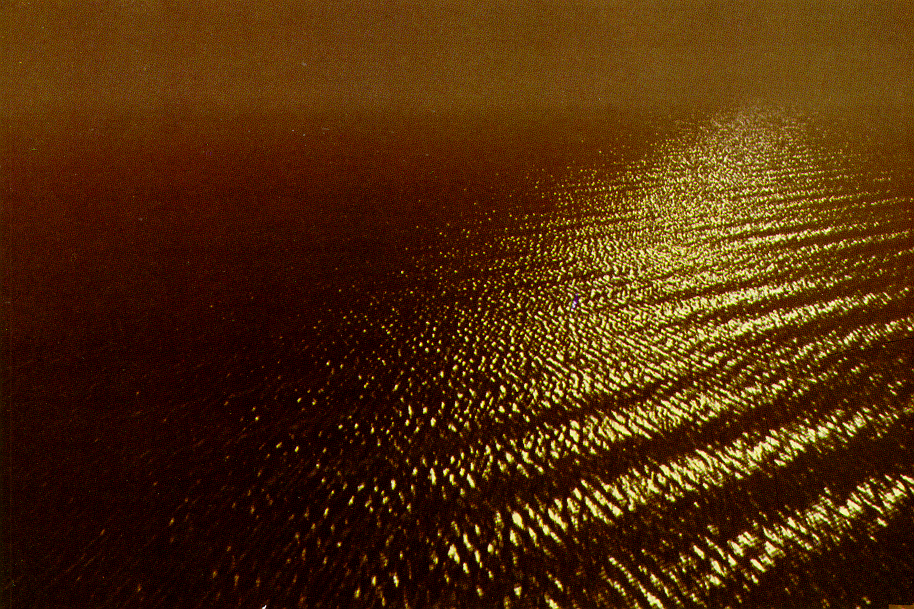
\includegraphics[scale=0.25]{figures/An_Image_Synthesizer_-_Perlin_1985-021.png}
 \caption{Perlin 1985}
\end{figure}

\begin{figure}
 \centering
 \subtop
 {
  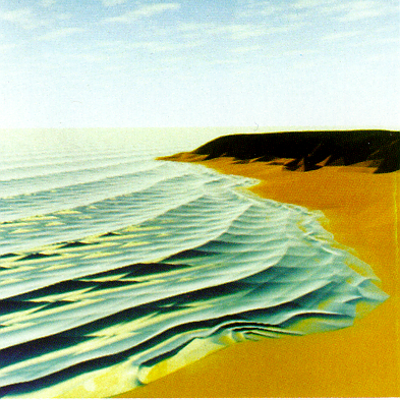
\includegraphics[scale=0.25]{figures/Modeling_Waves_and_Surf_-_Peachey_1986-009.png}
 }
 \hfill
 \subtop
 {
  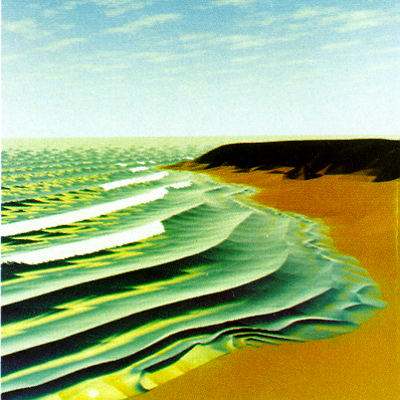
\includegraphics[scale=0.25]{figures/Modeling_Waves_and_Surf_-_Peachey_1986-010.png}
 }
 \hfill
 \subtop
 {
  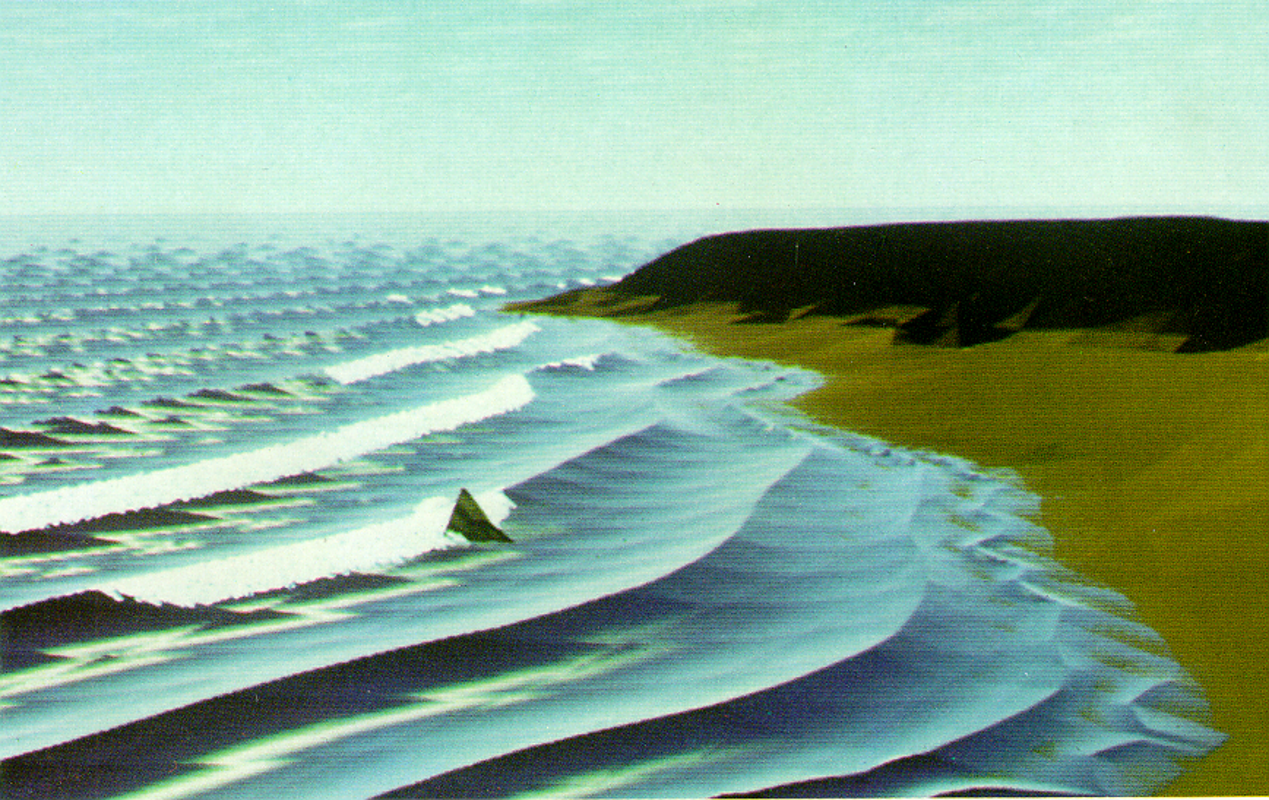
\includegraphics[scale=0.125]{figures/Modeling_Waves_and_Surf_-_Peachey_1986-012.png}
 }
 \caption{Peachey 1986}
\end{figure}

\begin{figure}
 \centering
 \subtop
 {
  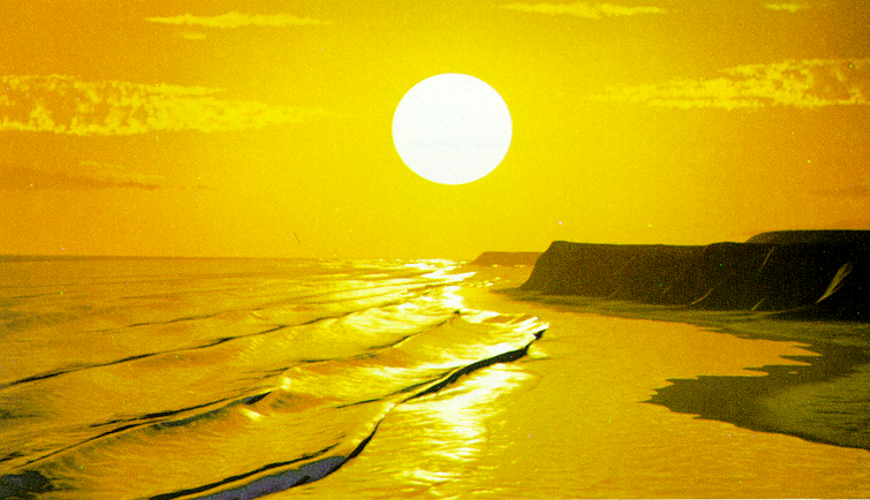
\includegraphics[scale=0.225]{figures/A_Simple_Model_of_Ocean_Waves_-_Fournier_1986-008.png}
 }
 \hfill
 \subtop
 {
  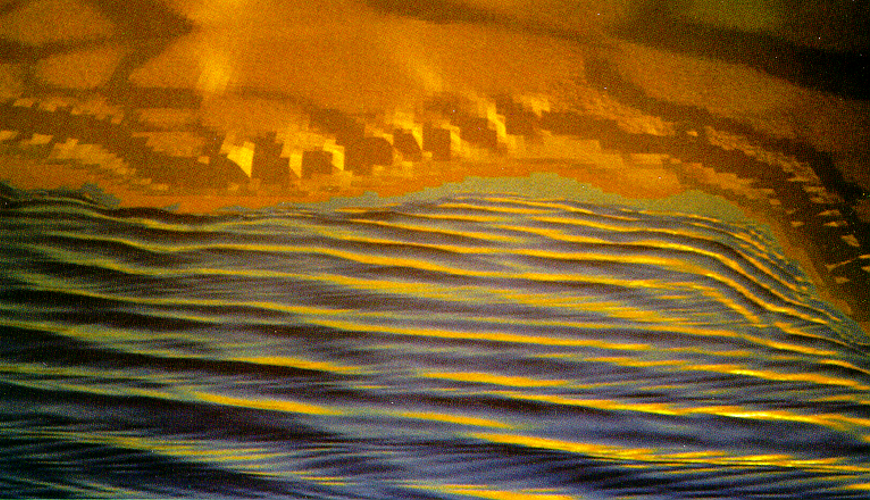
\includegraphics[scale=0.225]{figures/A_Simple_Model_of_Ocean_Waves_-_Fournier_1986-010.png}
 }
 \subtop
 {
  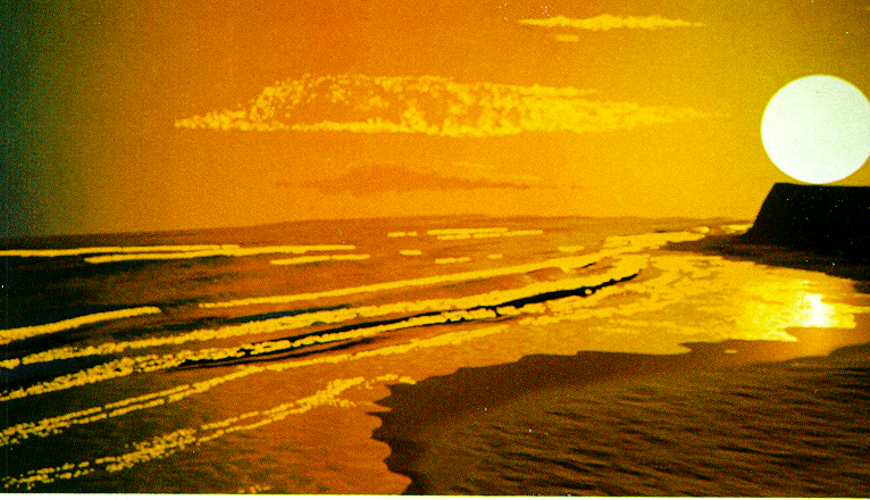
\includegraphics[scale=0.225]{figures/A_Simple_Model_of_Ocean_Waves_-_Fournier_1986-011.png}
 }
 \hfill
 \subtop
 {
  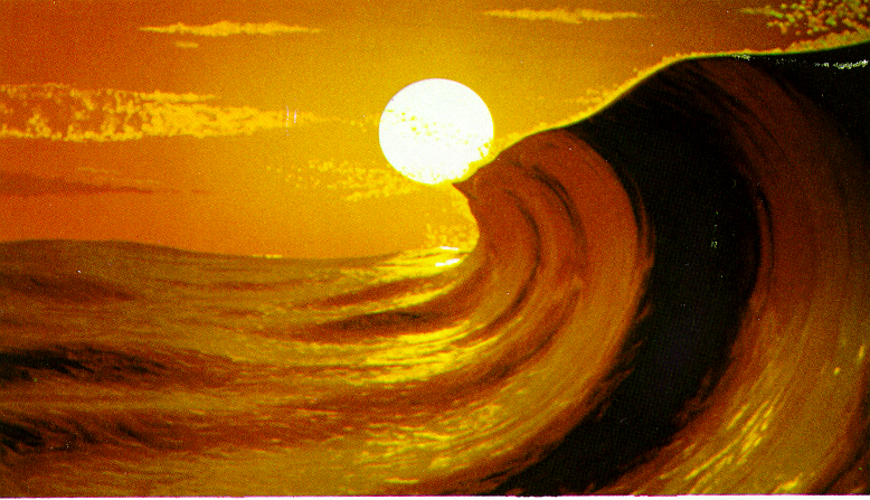
\includegraphics[scale=0.225]{figures/A_Simple_Model_of_Ocean_Waves_-_Fournier_1986-013.png}
	}
 \caption{Fournier 1986}
\end{figure}

\begin{figure}
 \centering
 \subtop
 {
  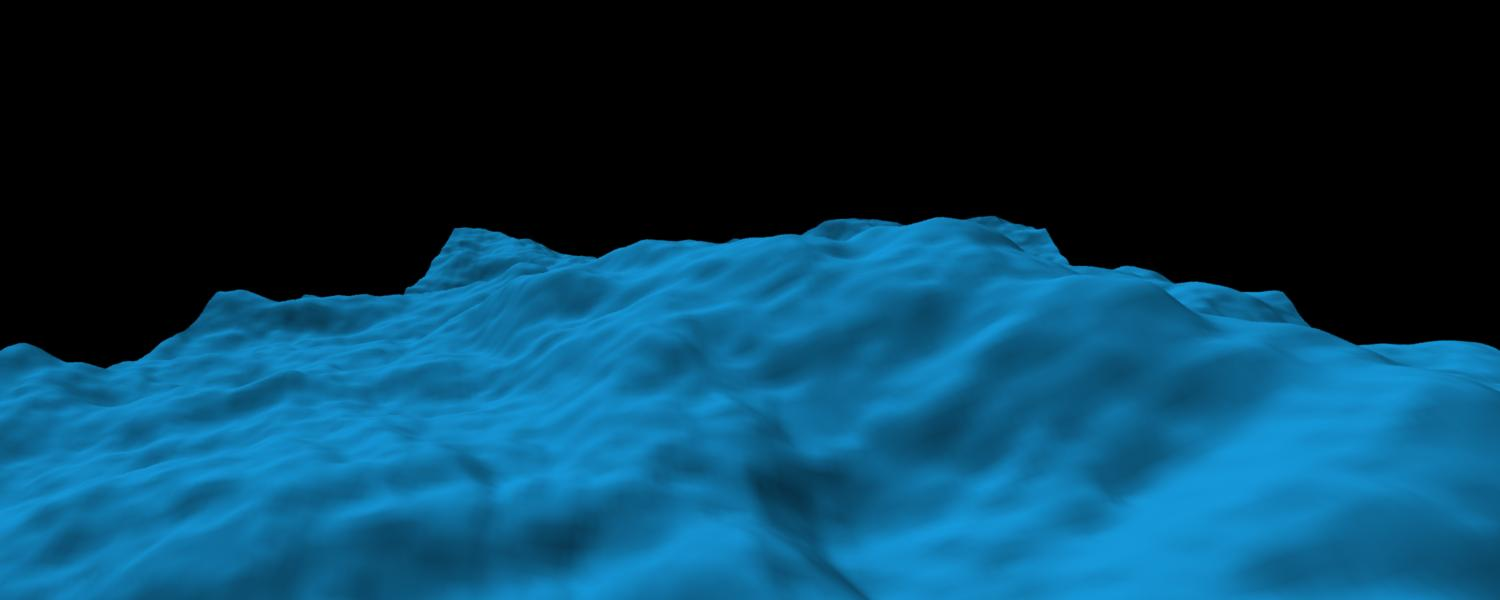
\includegraphics[scale=0.125]{figures/Simulating_Ocean_Water-012.png}
 }
 \subtop
 {
  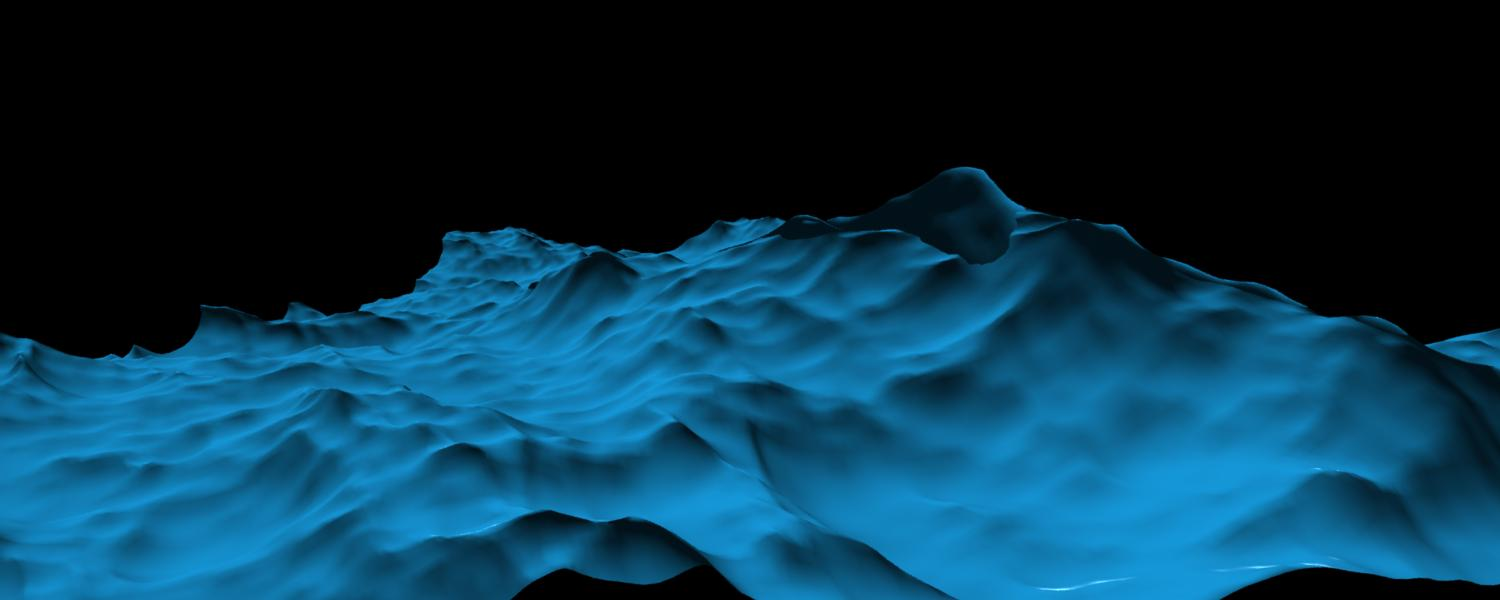
\includegraphics[scale=0.125]{figures/Simulating_Ocean_Water-013.png}
 }
 \caption{Tessendorf 1999}
\end{figure}

\begin{figure}
 \centering
 \subtop
 {
  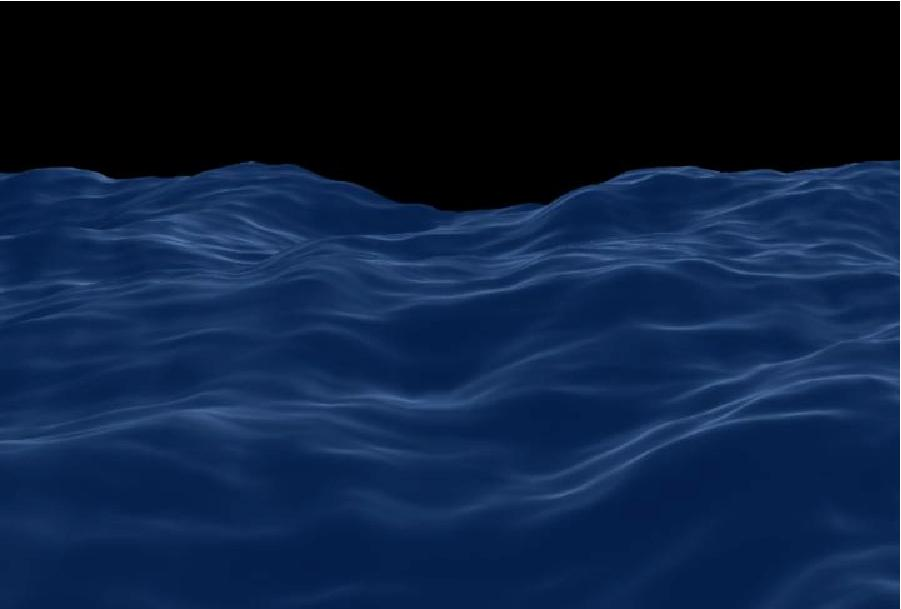
\includegraphics[scale=0.145]{figures/Simulating_Ocean_Water-008.png}
 }
 \hfill
 \subtop
 {
  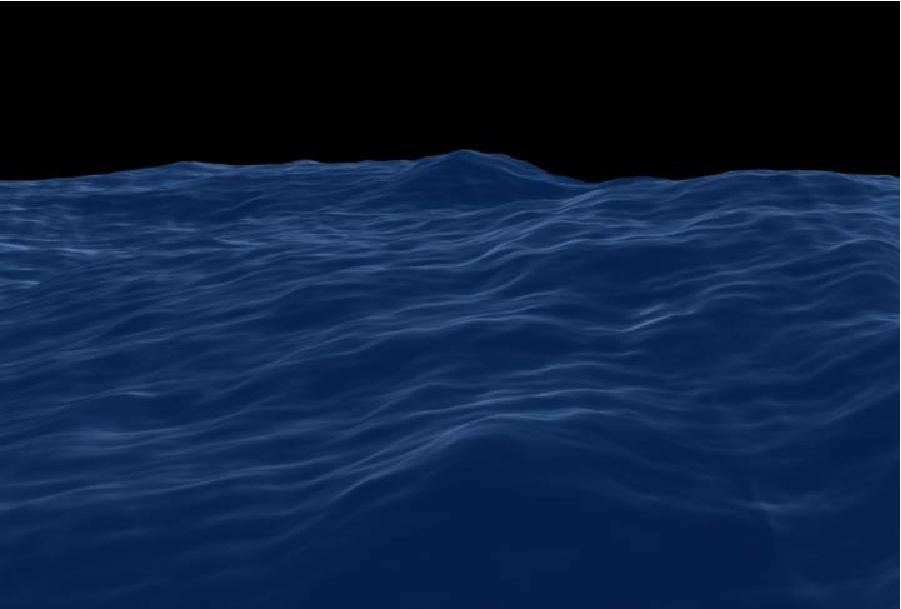
\includegraphics[scale=0.145]{figures/Simulating_Ocean_Water-009.png}
 }
 \hfill
 \subtop
 {
  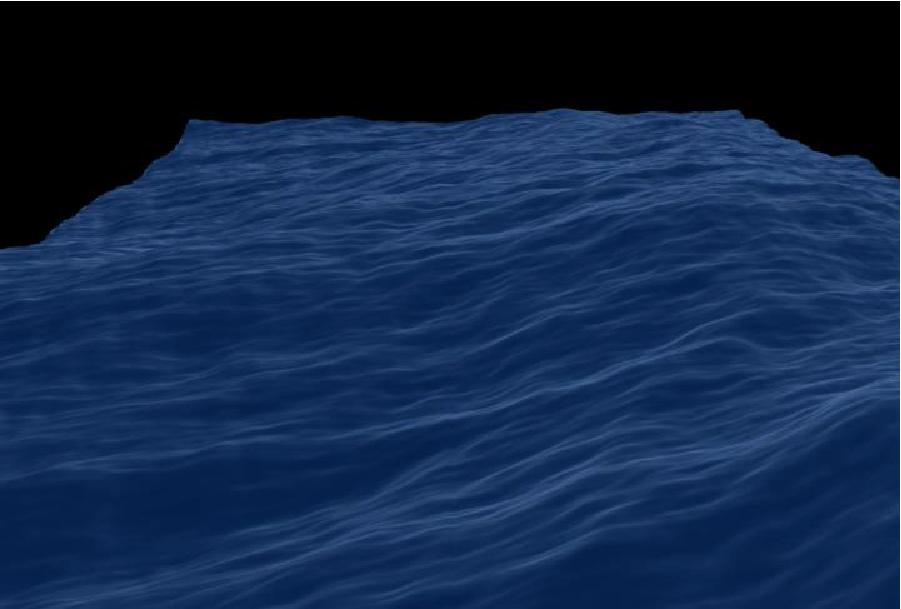
\includegraphics[scale=0.145]{figures/Simulating_Ocean_Water-010.png}
 }
 \caption{Tessendorf 1999}
\end{figure}